\documentclass[tikz,border=10pt]{standalone}
\usepackage{amsmath,amssymb}
\usetikzlibrary{arrows.meta,positioning,fit,backgrounds}
\begin{document}
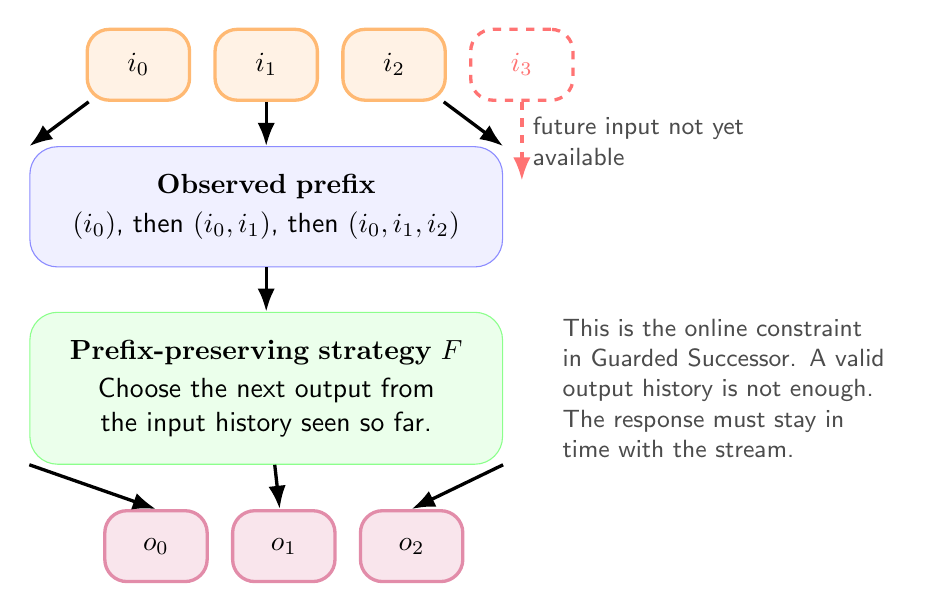
\begin{tikzpicture}[
  font=\sffamily,
  >=Latex,
  io/.style={draw, rounded corners=8pt, minimum width=1.3cm, minimum height=0.9cm, align=center, very thick},
  obs/.style={draw, rounded corners=10pt, fill=blue!6, draw=blue!45, align=center, inner sep=10pt, text width=5.3cm},
  strat/.style={draw, rounded corners=10pt, fill=green!8, draw=green!45, align=center, inner sep=10pt, text width=5.3cm},
  bad/.style={draw, rounded corners=8pt, minimum width=1.3cm, minimum height=0.9cm, align=center, very thick, dashed, draw=red!55, text=red!55},
  note/.style={font=\sffamily\small, align=left, text=black!70},
  arr/.style={->, very thick}
]

\node[io, fill=orange!10, draw=orange!55] (i0) {$i_0$};
\node[io, fill=orange!10, draw=orange!55, right=8pt of i0] (i1) {$i_1$};
\node[io, fill=orange!10, draw=orange!55, right=8pt of i1] (i2) {$i_2$};
\node[bad, right=8pt of i2] (i3) {$i_3$};

\node[obs, below=16pt of i1] (pref) {{\bf Observed prefix}\\[2pt]
$(i_0)$, then $(i_0,i_1)$, then $(i_0,i_1,i_2)$};

\node[strat, below=16pt of pref] (f) {{\bf Prefix-preserving strategy $F$}\\[2pt]
Choose the next output from the input history seen so far.};

\node[io, fill=purple!10, draw=purple!45, below=16pt of f, xshift=-1.4cm] (o0) {$o_0$};
\node[io, fill=purple!10, draw=purple!45, right=8pt of o0] (o1) {$o_1$};
\node[io, fill=purple!10, draw=purple!45, right=8pt of o1] (o2) {$o_2$};

\draw[arr] (i0) -- (pref.north west);
\draw[arr] (i1) -- (pref.north);
\draw[arr] (i2) -- (pref.north east);
\draw[arr] (pref) -- (f);
\draw[arr] (f) -- (o1);
\draw[arr] (f.south west) -- (o0.north);
\draw[arr] (f.south east) -- (o2.north);

\draw[->, dashed, red!55, very thick] (i3.south) -- ++(0,-1.0) node[midway,right, note, text width=2.9cm] {future input not yet available};

\node[note, right=18pt of f, text width=4.2cm] {
This is the online constraint in Guarded Successor. A valid output history is not enough. The response must stay in time with the stream.
};

\end{tikzpicture}
\end{document}
